%%
%% Commands for TeXCount
%TC:macro \cite [option:text,text]
%TC:macro \citep [option:text,text]
%TC:macro \citet [option:text,text]
%TC:envir table 0 1
%TC:envir table* 0 1
%TC:envir tabular [ignore] word
%TC:envir displaymath 0 word
%TC:envir math 0 word
%TC:envir comment 0 0
%%
%% The first command in your LaTeX source must be the \documentclass
%% command.
%%
%% For submission and review of your manuxscript please change the
%% command to \documentclass[manuscript, screen, review]{acmart}.
%%
%% When submitting camera ready or to TAPS, please change the command
%% to \documentclass[sigconf]{acmart} or whichever template is required
%% for your publication.
%%
%%
%\documentclass[manuscript,screen,review]{acmart}

\documentclass[sigconf,screen]{acmart}

%%
%% \BibTeX command to typeset BibTeX logo in the docs
\AtBeginDocument{%
  \providecommand\BibTeX{{%
    Bib\TeX}}}

%% Rights management information.  This information is sent to you
%% when you complete the rights form.  These commands have SAMPLE
%% values in them; it is your responsibility as an author to replace
%% the commands and values with those provided to you when you
%% complete the rights form.
\setcopyright{acmlicensed}
\copyrightyear{2026}
\acmYear{2026}
\acmDOI{XXXXXXX.XXXXXXX}
%% These commands are for a PROCEEDINGS abstract or paper.
\acmConference[Conference acronym 'XX]{Make sure to enter the correct
  conference title from your rights confirmation email}{June 03--05,
  2018}{Woodstock, NY}
%%
%%  Uncomment \acmBooktitle if the title of the proceedings is different
%%  from ``Proceedings of ...''!
%%
%%\acmBooktitle{Woodstock '18: ACM Symposium on Neural Gaze Detection,
%%  June 03--05, 2018, Woodstock, NY}
\acmISBN{978-1-4503-XXXX-X/2018/06}


%%
%% Submission ID.
%% Use this when submitting an article to a sponsored event. You'll
%% receive a unique submission ID from the organizers
%% of the event, and this ID should be used as the parameter to this command.
%%\acmSubmissionID{123-A56-BU3}

%%
%% For managing citations, it is recommended to use bibliography
%% files in BibTeX format.
%%
%% You can then either use BibTeX with the ACM-Reference-Format style,
%% or BibLaTeX with the acmnumeric or acmauthoryear sytles, that include
%% support for advanced citation of software artefact from the
%% biblatex-software package, also separately available on CTAN.
%%
%% Look at the sample-*-biblatex.tex files for templates showcasing
%% the biblatex styles.
%%

%%
%% The majority of ACM publications use numbered citations and
%% references.  The command \citestyle{authoryear} switches to the
%% "author year" style.
%%
%% If you are preparing content for an event
%% sponsored by ACM SIGGRAPH, you must use the "author year" style of
%% citations and references.
%% Uncommenting
%% the next command will enable that style.
%%\citestyle{acmauthoryear}


\usepackage{tabularx}
\usepackage{comment}
\usepackage[normalem]{ulem}


% --- Algorithms ---
\usepackage{algorithm}

\usepackage[noend]{algpseudocode}
\algrenewcommand\algorithmicrequire{\textbf{Input:}}
\algrenewcommand\algorithmicensure{\textbf{Output:}}
\floatname{algorithm}{Algorithm}

% --- TikZ + scaling support ---
\usepackage{tikz}
\usetikzlibrary{arrows.meta, calc, positioning, fit, backgrounds, shapes.geometric}
\usepackage{adjustbox}  % <--- prevents figure overflow

\usepackage{xcolor}
\usepackage{graphicx}
\usepackage{subcaption}
 \usepackage{multirow}


% --- tcolorbox ---
\usepackage[most]{tcolorbox}
% Default tcolorbox: always fit inside the text width
\tcbset{
    width=\linewidth,
    colback=gray!10,
    colframe=gray!60,
    boxrule=0.5pt,
    arc=3pt,
    left=8pt, right=8pt, top=6pt, bottom=6pt,
}

% --- Prevent TikZ figures from overflowing ---
% Wrap any oversized tikzpicture inside adjustbox automatically
\newenvironment{tikzboxed}
{\begin{adjustbox}{max width=\linewidth}\begin{tikzpicture}}
{\end{tikzpicture}\end{adjustbox}}


\newcommand\Logan[1]{\leavevmode{\footnotesize\textbf{[Logan: #1]}}}


%%
%% end of the preamble, start of the body of the document source.
\begin{document}

%%
%% The "title" command has an optional parameter,
%% allowing the author to define a "short title" to be used in page headers.
\title{Energy-Efficient Embedded Cybersecurity for Satellite Avionics}

%%
%% The "author" command and its associated commands are used to define
%% the authors and their affiliations.
%% Of note is the shared affiliation of the first two authors, and the
%% "authornote" and "authornotemark" commands
%% used to denote shared contribution to the research.
\author{Sirio Jansen-Sánchez}
\email{jansenss@my.erau.edu}
\orcid{0009-0001-6498-418X}
\authornote{These authors contributed equally to this work.}
\affiliation{%
  \institution{Embry-Riddle Aeronautical University}
\city{Daytona Beach}
  \state{Florida}
  \country{USA}
}
\author{Logan Luna}
\email{lambethl@my.erau.edu}
\orcid{0009-0001-0713-4074}
\authornotemark[1]
%\email{webmaster@marysville-ohio.com}
\affiliation{%
  \institution{Embry-Riddle Aeronautical University}
  \city{Daytona Beach}
  \state{Florida}
  \country{USA}
}
\author{Joseph Rigo}
\email{rigoj1@my.erau.edu}
\orcid{0009-0007-9844-9672}
%\email{webmaster@marysville-ohio.com}
\affiliation{%
  \institution{Embry-Riddle Aeronautical University}
\city{Daytona Beach}
  \state{Florida}
  \country{USA}
}
\author{Author}
\email{trovato@corporation.com}
\orcid{1234-5678-9012}
\email{webmaster@marysville-ohio.com}
\affiliation{%
  \institution{Embry-Riddle Aeronautical University}
\city{Daytona Beach}
  \state{Florida}
  \country{USA}
}
\author{Author}
\email{trovato@corporation.com}
\orcid{1234-5678-9012}
\email{webmaster@marysville-ohio.com}
\affiliation{%
  \institution{Embry-Riddle Aeronautical University}
\city{Daytona Beach}
  \state{Florida}
  \country{USA}
}

%%
%% The abstract is a short summary of the work to be presented in the
%% article, 100 words.
\begin{abstract}
Satellites serve as essential communication backbones for distributed energy infrastructure; however, their onboard networks are often insufficiently protected against cyberattacks. We introduce a lightweight intrusion detection system (IDS) for satellite Controller Area Network (CAN) bus traffic, occupying 541 bytes of flash memory and executing in 4.2 microseconds on an STM32F373C8T microcontroller operating at 72 MHz. Our system extracts 14 domain-specific CAN features and implements a depth-5 decision tree as static C arrays without heap allocation. Comprehensive hardware firmware validation across 348,000 classified frames demonstrates the following results: for native satellite CAN traffic, the IDS achieves 99.86\% recall and 0.9912 ROC-AUC across four attack classes (DoS, Fuzzy, Spoofing, Replay); for UNSW-NB15 encoded as CAN streams, 93.64\% recall and 69.97\% F1; and for NSL-KDD, 52.88\% recall, 86.65\% precision, and 65.68\% F1 with a 10.76\% false positive rate. Concurrent SATLL EPS telemetry quantifies the IDS power consumption at two levels. The inference increment, representing the marginal algorithmic cost at 100 Hz, is at most 48–53 microWatts (upper bound: $I_\text{base} \times V_{dd} \times t_\text{inf} \times f_\text{poll}$, measured $I_\text{base} = 35\text{--}38$~mA), which is less than 0.004\% of the 1,273 mW ADCS overhead during sensor experiments. The complete evaluation board draws 164–176 mW from the satellite payload port (115–125 mW for constant MCU active-run, approximately 49 mW for the USB bridge and peripherals). This overhead can be eliminated through native OBDH integration, reducing the residual IDS cost to approximately 40 microWatts.\end{abstract}

%%
%% The code below is generated by the tool at http://dl.acm.org/ccs.cfm.
%% Please copy and paste the code instead of the example below.
%%
\begin{CCSXML}
<ccs2012>
   <concept>
       <concept_id>10002978.10002997.10002999</concept_id>
       <concept_desc>Security and privacy~Intrusion detection systems</concept_desc>
       <concept_significance>500</concept_significance>
       </concept>
   <concept>
       <concept_id>10002978.10003001.10003003</concept_id>
       <concept_desc>Security and privacy~Embedded systems security</concept_desc>
       <concept_significance>500</concept_significance>
       </concept>
   <concept>
       <concept_id>10010583.10010662.10010668</concept_id>
       <concept_desc>Hardware~Energy distribution</concept_desc>
       <concept_significance>500</concept_significance>
       </concept>
   <concept>
       <concept_id>10010583.10010662.10010674</concept_id>
       <concept_desc>Hardware~Power estimation and optimization</concept_desc>
       <concept_significance>500</concept_significance>
       </concept>
 </ccs2012>
\end{CCSXML}

\ccsdesc[500]{Security and privacy~Intrusion detection systems}
\ccsdesc[500]{Security and privacy~Embedded systems security}
\ccsdesc[500]{Hardware~Energy distribution}
\ccsdesc[500]{Hardware~Power estimation and optimization}


%\ccsdesc[500]{Do Not Use This Code~Generate the Correct Terms for Your Paper}
%\ccsdesc[300]{Do Not Use This Code~Generate the Correct Terms for Your Paper}
%\ccsdesc{Do Not Use This Code~Generate the Correct Terms for Your Paper}
%\ccsdesc[100]{Do Not Use This Code~Generate the Correct Terms for Your Paper}

%%
%% Keywords. The author(s) should pick words that accurately describe
%% the work being presented. Separate the keywords with commas.
\keywords{Words}

\received{20 February 2007}
\received[revised]{12 March 2009}
\received[accepted]{5 June 2009}

%%
%% This command processes the author and affiliation and title
%% information and builds the first part of the formatted document.
\maketitle

% \tableofcontents

\input{content/introduction}

% Feature importance figure spans both columns — place before \section so LaTeX
% can float it to the top of the methodology page.
\begin{figure*}[t]
    \centering
    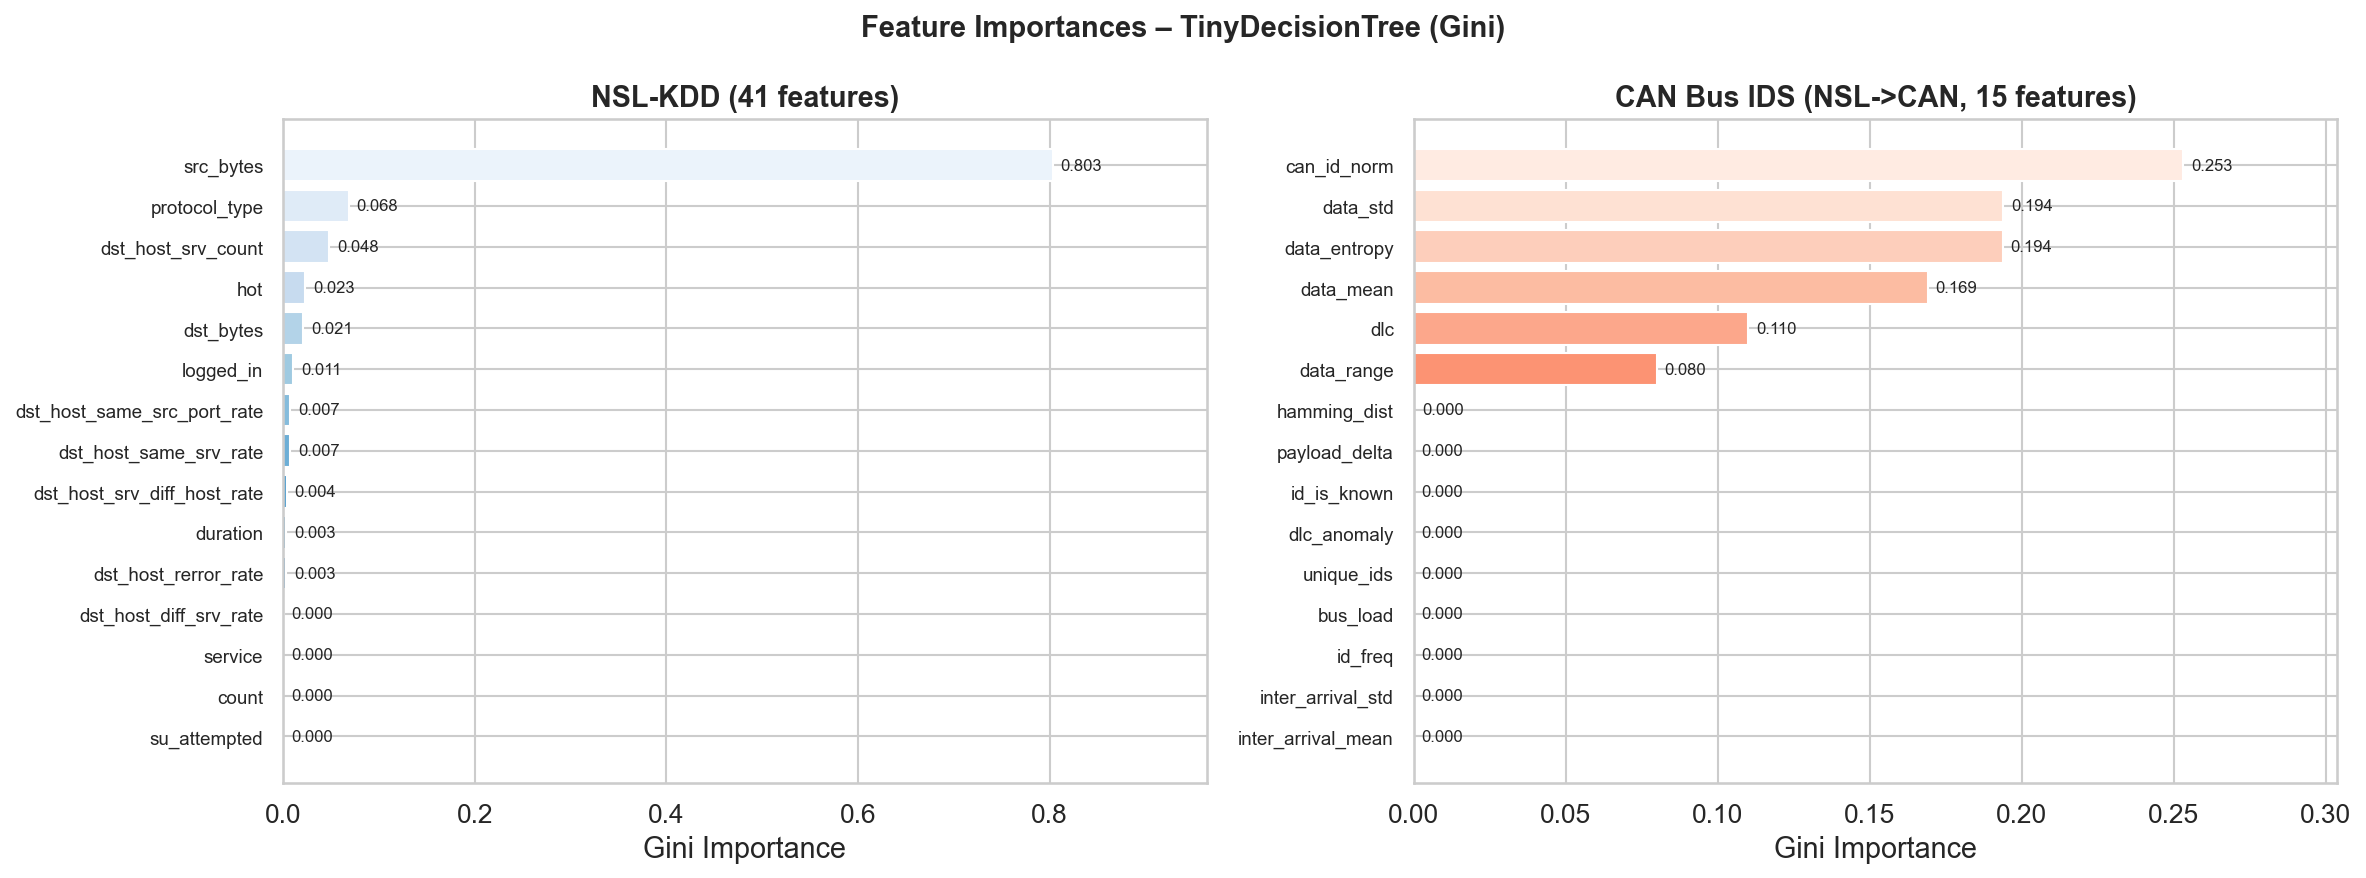
\includegraphics[width=\linewidth]{images/09_feature_importance.png}
    \caption{Gini impurity importances for the deployed TinyDecisionTree on NSL-KDD (left, 41 network features) and the Satellite CAN IDS (right, 15 CAN features).}
    \label{fig:feature_importance}
\end{figure*}

% ------------------------------------------------------------------
\section{Methodology}
\label{sec:methodology}
% ------------------------------------------------------------------

In the following section we describe the five-stage pipeline we have developed from training to inference. All computationally intensive tasks, including dataset generation, feature extraction, model training, threshold analysis, quantization, and C-code export, are conducted offline using ground infrastructure. The microcontroller is responsible solely for executing a bounded, heap-free inference path. To maintain clarity and reproducibility, we organize the paper such that all methodological details, including the design of our five-stage pipeline, candidate model selection, and offline benchmarking, are presented in this section. In Section~\ref{sec:results}, we present the results of the deployed system, focusing on online evaluation, hardware performance, and live experimental outcomes.

\begin{comment}
    
\subsection{End-to-End Pipeline}

The system implements a five-stage pipeline that enforces a strict separation between ground-side training and onboard inference. All computationally intensive tasks, including dataset generation, feature extraction, model training, threshold analysis, quantization, and C-code export, are conducted offline using ground infrastructure. The microcontroller is responsible solely for executing a bounded, heap-free inference path.

\begin{enumerate}
    \item \textbf{CAN traffic generation.} Labeled satellite CAN bus traffic is produced by the SATLL hardware under two controlled experimental regimes (Section~\ref{sec:experiments}), with synthetic attack injections applied at controlled rates.
    \item \textbf{Feature extraction.} A sliding window of 50 frames is maintained as frames arrive; 14 features are computed per frame.
    \item \textbf{Model training and selection.} Five candidate classifiers are benchmarked; the depth-constrained decision tree is selected for its sub-kilobyte flash footprint and sub-microsecond latency.
    \item \textbf{Quantization-aware export.} The trained tree and scaler parameters are exported as static C arrays in three numeric formats (float32, int16, int8) for flash-footprint comparison.
    \item \textbf{Firmware integration.} The C header is linked into a STM32 build. Inference is driven by the host-side runner over USB OTG (CDC ACM) for benchmarking; onboard autonomous monitoring is the operational target.
\end{enumerate}

\end{comment}


% ------------------------------------------------------------------
\subsection{CAN Feature Engineering}
\label{sec:features}
% ------------------------------------------------------------------

A total of fourteen features are extracted from an offline 50-frame sliding window over the raw CAN bus stream. These features are categorized as payload structure, temporal dynamics, and bus topology, as detailed in Table~\ref{tab:features}. The sliding window maintains per-ID history, ensuring that per-ID timing statistics remain computable even in a shared bus environment.

Scaling parameters ($\mu$, $\sigma$) are estimated from the training corpus and stored as 30 float32 constants (120 bytes) alongside the decision tree. During inference, each feature value is z-scored using these constants prior to tree evaluation.

% ------------------------------------------------------------------
\subsection{Candidate Model Evaluation and Selection}
\label{sec:model_selection}
% ------------------------------------------------------------------

Five model architectures are benchmarked on real-world network-IDS datasets (UNSW-NB15 and NSL-KDD \cite{UNSW2015, NSLKDD2009}) to establish the trade-off between resource usage and accuracy prior to domain-specific CAN training. The evaluated candidates include a shallow TinyDecisionTree (depth $\leq$ 5), TinyXGBoost and MicroXGBoost (with 3 and 5 gradient-boosted trees, respectively), a LightRandomForest (10 trees), and a CompactExtraTrees ensemble (8 trees). Each model is assessed based on recall, F1-score, ROC-AUC, serialized flash size, and per-sample inference latency. Comprehensive benchmark results are presented in Table~\ref{tab:model_comparison}. On UNSW-NB15 all models achieve similarly high recall ($\geq$98.9\%), so the differentiating axes are flash footprint and inference latency. The ensemble methods (LightRandomForest at 106~KB, CompactExtraTrees at 41~KB) are immediately eliminated by the CubeSat flash constraint; their 14\,ms per-sample latency would consume an impractical share of the OBDH task budget. MicroXGBoost and TinyXGBoost occupy 6--10~KB and 260--320~\textmu s—below the flash threshold but two orders of magnitude slower than the decision tree. On NSL-KDD, TinyXGBoost achieves slightly higher recall (69.2\% vs 65.7\%) but at the cost of 10$\times$ the inference time.

TinyDecisionTree is the only model meeting all three embedded constraints simultaneously: $<$6~KB serialized size, $<$30~\textmu s inference on host CPU, and recall $\geq$65\% across both datasets. It is selected for all subsequent CAN-domain training and firmware integration.

\begin{table}[t]
\caption{All candidate models on UNSW-NB15 and NSL-KDD real-world benchmarks. \textbf{Bold}: selected for embedded deployment. Latency measured on host CPU.}
\label{tab:model_comparison}
\small
\begin{tabular}{@{}llrrrrr@{}}
\toprule
\textbf{Model} & \textbf{Dataset} & \textbf{Rec.} & \textbf{F1} & \textbf{AUC} & \textbf{Size} & \textbf{Lat.} \\
               &                  & (\%)          & (\%)        &              & (KB)          & (\textmu s)   \\
\midrule
\multirow{2}{*}{\textbf{TinyDecisionTree}}
  & UNSW-NB15 & \textbf{99.4} & \textbf{85.2} & 0.930 & \textbf{5.1}  & \textbf{29} \\
  & NSL-KDD   & \textbf{65.7} & \textbf{78.1} & 0.795 & \textbf{5.2}  & \textbf{29} \\
\midrule
\multirow{2}{*}{TinyXGBoost}
  & UNSW-NB15 & 99.5 & 81.5 & 0.863 & 6.6 & 262 \\
  & NSL-KDD   & 69.2 & 80.0 & 0.896 & 6.6 & 318 \\
\midrule
\multirow{2}{*}{MicroXGBoost}
  & UNSW-NB15 & 99.8 & 83.0 & 0.927 & 9.7 & 259 \\
  & NSL-KDD   & 65.0 & 77.6 & 0.920 & 9.7 & 272 \\
\midrule
\multirow{2}{*}{LightRandomForest}
  & UNSW-NB15 & 99.6 & 85.1 & 0.969 & 106.4 & 14{,}287 \\
  & NSL-KDD   & 65.3 & 78.0 & 0.948 & 118.3 & 14{,}545 \\
\midrule
\multirow{2}{*}{CompactExtraTrees}
  & UNSW-NB15 & 98.9 & 83.2 & 0.880 & 41.3 & 14{,}721 \\
  & NSL-KDD   & 60.1 & 74.6 & 0.886 & 58.7 & 14{,}517 \\
\bottomrule
\end{tabular}
\end{table}

% ------------------------------------------------------------------

% ------------------------------------------------------------------
\subsection{Satellite CAN IDS Training}
\label{sec:can_training}
% ------------------------------------------------------------------

The TinyDecisionTree model is retrained from scratch using the satellite CAN dataset. The training set consists of 25,861 feature vectors derived from labeled satellite CAN frames, while 5,166 held-out frames form the offline test set, with approximately 54.7% attack class representation in each split. The attack class labels include four categories that represent established CAN bus intrusion techniques:

\begin{itemize}
    \item \textbf{DoS}: burst-flooding that saturates the bus
    \item \textbf{Fuzzy}: random-payload injection across all IDs
    \item \textbf{Spoofing}: injection of valid-looking frames under a legitimate ID
    \item \textbf{Replay}: re-transmission of previously captured normal frames
\end{itemize}

The decision tree is limited to a depth of five, resulting in 39 nodes and 20 leaves (Figure~\ref{fig:tree_structure}). Training completes in 57 ms, and the exported C header file is 541 bytes in size. On the offline held-out set, the model achieves 99.86% recall and a 0.9912 ROC-AUC across all four attack classes.

For cross-domain evaluation, the UNSW-NB15 dataset (82,000 test flows, 34 features) and the NSL-KDD dataset (22,000 test samples, 41 features, including 17 previously unseen attack types) are serialized as synthetic CAN streams and processed through the same 14-feature extraction pipeline (Algorithm~\ref{alg:b2can}, Appendix~\ref{app:b2can}). On UNSW-NB15, the offline decision tree achieves 99.43\% recall and a 0.9301 AUC; on NSL-KDD, it achieves 65.73\% recall and a 0.7951 AUC. Figure~\ref{fig:feature_importance} presents the relative feature importances in both domains, Figure~\ref{fig:roc_curves} displays the ROC curves, and Figure~\ref{fig:radar_summary} summarizes the overall model performances.

\begin{figure}[t]
    \centering
    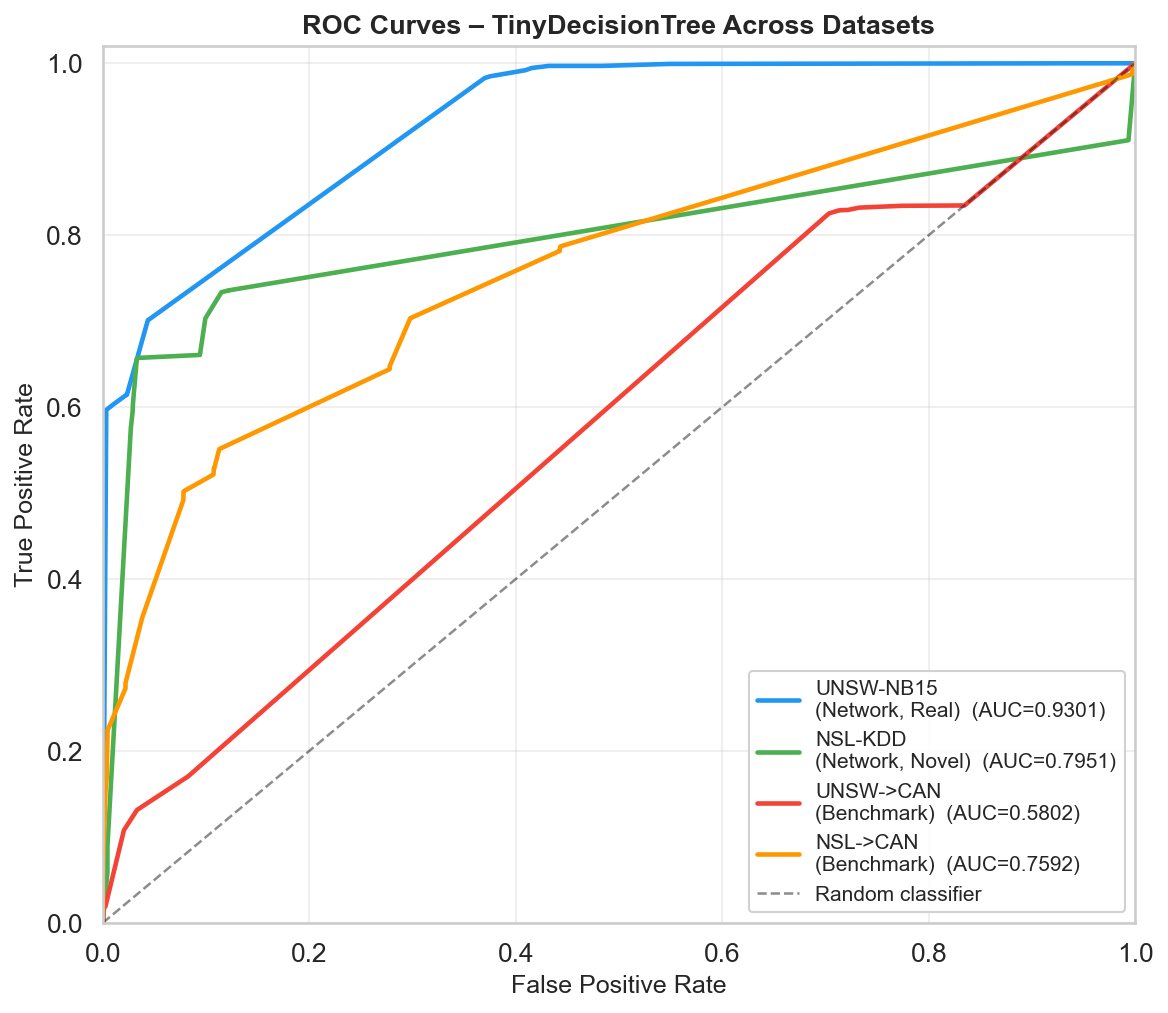
\includegraphics[width=\linewidth]{images/10_roc_curves.png}
    \caption{ROC curves for TinyDecisionTree across deployment domains.}
    \label{fig:roc_curves}
\end{figure}

\begin{figure}
    \centering
    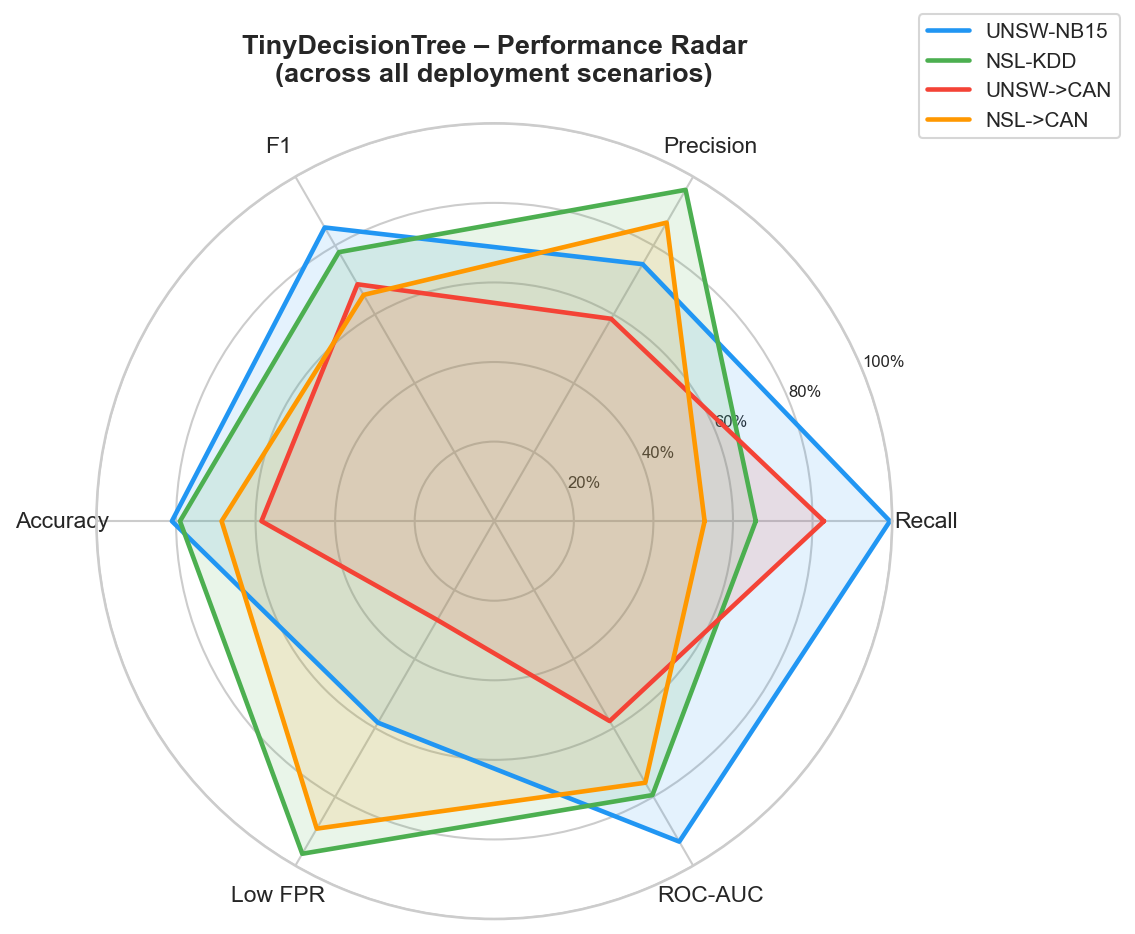
\includegraphics[width=\linewidth]{images/11_radar_summary.png}
    \caption{Radar summary comparing the performance of TinyDecisionTree before and after datasets and benchmarks are converted to CAN format.}
    \label{fig:radar_summary}
\end{figure}

\subsubsection{Benchmark-to-CAN Encoding}

Tabular benchmark samples are serialized as synthetic CAN frame streams. Each stream begins with a meta frame containing the sample index and label, followed by $\lceil F/8 \rceil$ payload frames with min-max-scaled uint8 feature bytes. These streams are then processed through the same 14-feature extraction pipeline as native traffic (Algorithm~\ref{alg:b2can}, Appendix~\ref{app:b2can}). The resulting domain shift quantifies the gap between models trained on network intrusion detection system benchmarks and those deployed in authentic satellite CAN environments.

% ------------------------------------------------------------------
\subsection{Quantization and Model Export}
\label{sec:quantization}
% ------------------------------------------------------------------

Three numeric precision variants of the trained tree are exported as self-contained C headers: Float32 (32-bit IEEE thresholds), Int16 (linearly quantized), and Int8. Float32 is selected for deployment; Int16 is retained as a Cortex-M0/M0+ fallback. Detailed size, latency, and detection-quality comparisons across formats are provided in Appendix~\ref{app:quantization}.


% ------------------------------------------------------------------
\subsection{Firmware Integration and Host-Side Runner}
\label{sec:firmware}
% ------------------------------------------------------------------

For hardware-in-the-loop deployment, the Zubax CANFace CF1 "Babel" served as the CAN-to-host bridge \cite{ZubaxBabelShop2026}. The experimental setup imposed strict constraints on receive buffering, limited to approximately three frames, which required deterministic and lightweight online processing. To meet these requirements, the open-source CANFace CF1 firmware stack \cite{ZubaxCanfaceCF1Repo2026} was modified by replacing the default SLCAN parsing and wrapping path with an inference-oriented acquisition and analysis path specifically designed for IDS benchmarking.

During benchmarking, the STM32 evaluation board is powered by the SATLL payload 5 V rail. A host-side runner streams pre-extracted feature vectors via USB OTG (CDC ACM), while the microcontroller unit (MCU) returns the prediction label, DWT cycle count, and stack high-water mark for each sample. The protocol is detailed in Appendix~\ref{app:protocol}.

Power consumption is measured using SATLL EPS housekeeping telemetry ($P = V_{\text{payload}} \cdot I_{\text{payload}}$), which is logged at 1 Hz. Two quantities are distinguished: the board-level draw, representing the full STM32 evaluation board on the payload rail, and the inference increment, which is the marginal cost of tree traversal alone, bounded by:
\[
    \Delta P_{\text{IDS}} \leq I_{\text{base}} \cdot V_{\text{DD}} \cdot t_{\text{inf}} \cdot f_{\text{poll}},
\]
where $I_{\text{base}}=35$--$38$~mA (measured), $V_{\text{DD}}=3.3$~V, $t_{\text{inf}} \approx 4.2$~\textmu s, and $f_{\text{poll}}=100$~Hz. Complete power measurement results are provided in Section~\ref{sec:res_power}.

% ------------------------------------------------------------------
\subsection{SATLL Experimental Protocol}
\label{sec:experiments}
% ------------------------------------------------------------------

A live evaluation is conducted on the KISPE SATLL using two distinct subsystem experiments. Each experiment comprises two phases: a clean baseline collection phase to characterize normal traffic, followed by an attack injection phase. Attacks are introduced at controlled rates by a separate CAN node connected to the shared bus. The IDS operates continuously during both phases and records labels with microsecond-resolution timestamps.

\subsubsection{Accelerometer Experiment}

The Accelerometer experiment is conducted as part of the Attitude Determination and Control System (ADCS), with a specific focus on the attitude determination component. The objective of this experiment is to demonstrate changes in acceleration across the x, y, and z axes. The satellite's attitude determination capabilities are evaluated by observing varying acceleration values as its position and angle are adjusted. This test is considered effective because it yields relatively stable values for each angle and orientation, resulting in consistent data suitable for research purposes.


\subsubsection{Reaction Wheel Experiment}

The Reaction Wheel experiment is also conducted within the ADCS framework. While it incorporates aspects of attitude determination, its primary emphasis is on the control system. This experiment demonstrates the reaction wheel's operation by spinning the satellite upon activation. As the satellite rotates, corresponding changes in gyro values are observed. The experiment thus evaluates both the satellite’s capability to alter its orientation and to track these changes. Although the data obtained are less consistent than those from the Accelerometer experiment, due to satellite swinging during operation, the test provides a solid foundation and a distinct dataset for further analysis.

% ------------------------------------------------------------------
\section{Results}
\label{sec:results}

% ------------------------------------------------------------------
\subsection{Hardware Firmware Validation}
\label{sec:res_hardware}
% ------------------------------------------------------------------

The exported model undergoes end-to-end validation on an STM32F373C8T microcontroller operating at 72 MHz using the UART/USB-OTG CDC-ACM benchmark protocol. Table~\ref{tab:hardware} presents the measured resource utilization and timing results for both cross-domain test sets.

\begin{table}[t]
\caption{STM32F373C8T hardware benchmark at 72 MHz and 3.3 V. The flash memory includes tree decision arrays (429 B) and a feature scaler (112 B). Machine learning performance is evaluated on the respective cross-domain test sets. Power analysis results are provided in Table~\ref{tab:power}.}
\label{tab:hardware}
\small
\begin{tabular}{@{}lrr@{}}
\toprule
\textbf{Metric} & \textbf{UNSW-NB15} & \textbf{NSL-KDD} \\
\midrule
Flash (tree + scaler)        & \multicolumn{2}{c}{541~B (0.53~KB)} \\
RAM (feature buffer)         & \multicolumn{2}{c}{60~B (stack only)} \\
Heap                         & \multicolumn{2}{c}{none (bare-metal)} \\
\midrule
Cycles (mean)                & 301.7 & 302.9 \\
Inference mean               & 4.19~\textmu s & 4.21~\textmu s \\
Inference p99                & 4.24~\textmu s & 4.24~\textmu s \\
CPU duty @ 100~Hz            & \multicolumn{2}{c}{0.042\%} \\
\midrule
Samples classified           & 300,000        & 48,000 \\
Accuracy (\%)                & 55.75          & 68.55 \\
Recall (\%)                  & 93.64          & 52.88 \\
Precision (\%)               & 55.85          & 86.65 \\
F1 (\%)                      & 69.97          & 65.68 \\
FPR (\%)                     & 90.68          & 10.76 \\
\bottomrule
\end{tabular}
\end{table}

The flash memory footprint is 541 bytes, comprising 429 bytes for tree arrays and 112 bytes for the scaler. RAM usage consists of a stack-allocated 60-byte \texttt{float[14]} buffer, with no heap allocation. Inference completes in 4.19 to 4.21 microseconds (300 to 303 cycles) across both datasets; the p99 latency is 4.24 microseconds, demonstrating deterministic and bounded execution over 348,000 cumulative inferences. The variance of less than 0.015 microseconds is attributable to the fixed-depth structure, as each classification traverses a single root-to-leaf path. At a polling rate of 100 Hz, the intrusion detection system utilizes 0.042\% of the CPU. Power analysis results are detailed in Section~\ref{sec:res_power}.

% ------------------------------------------------------------------
\subsection{Cross-Domain Generalization}
\label{sec:res_crossdomain}
% ------------------------------------------------------------------

The hardware results in Table~\ref{tab:hardware} quantify out-of-domain performance when the model trained on native satellite CAN traffic classifies benchmark network flows encoded as CAN frames. On the NSL-KDD dataset, the firmware achieves 52.88\% recall and 10.76\% false positive rate (FPR), correctly identifying approximately half of the 31 attack types while maintaining a manageable false positive rate. For UNSW-NB15, recall increases to 93.64\%, but the FPR rises to 90.68\%, suggesting that the class boundary learned from CAN telemetry is excessively permissive given this dataset's class distribution (55\% attack).

The per-attack breakdown for NSL-KDD (Table~\ref{tab:per_attack_full}, Appendix) demonstrates the anticipated pattern: anomaly-based attacks that modify payload statistics (buffer\_overflow: 52\%, rootkit: 55\%, xlock: 57\%) are detected at rates above the mean recall of 35\%. In contrast, purely semantic attacks with structurally normal payloads (xterm: 7\%, sendmail: 10\%, xsnoop: 10\%) achieve near-zero detection rates. These results indicate that the satellite CAN feature set captures meaningful signal structure even from unfamiliar traffic, but also highlight the necessity of training on mission-representative data for effective production deployment.


% ------------------------------------------------------------------
\subsection{Power Budget Analysis}
\label{sec:res_power}
% ------------------------------------------------------------------

Power consumption was characterized across five SATLL sessions encompassing three operational states: platform idle (baseline), sensor experiments (accelerometer and reaction wheel), and IDS benchmark runs (NSL-KDD and UNSW-NB15). EPS housekeeping telemetry was recorded at one-second intervals, and per-rail power was calculated from decoded CDH fields using $P = V \times I$. The STM32F373C8T evaluation board received power from the SATLL payload 5 V rail during all IDS sessions, allowing the payload rail to directly reflect total board consumption. Table~\ref{tab:power} provides the per-session, per-rail breakdown and details the decomposition of board consumption into MCU base, board peripherals, and the IDS inference-specific increment.

\begin{table*}[t]
\caption{SATLL per-rail power (mean mW) across all five sessions derived from EPS telemetry, with IDS board decomposition for the benchmark runs.}
\label{tab:power}
\small
\setlength{\tabcolsep}{3pt}
\begin{tabular}{@{}lrrrrr@{}}
\toprule
\textbf{Component} & \textbf{Baseline} & \textbf{Accel.} & \textbf{Rx Wheel} & \textbf{NSL run} & \textbf{UNSW run} \\
\midrule
\multicolumn{6}{@{}l}{\textit{SATLL platform rails (mW)}} \\
System total          & 1,608 & 2,881 & 3,078 & 1,792 & 1,835 \\
OBC                   &   968 &   975 &   975 &   980 &   986 \\
Platform 5~V          & 1,298 & 1,300 & 1,302 & 1,304 & 1,313 \\
Comms                 &   295 &   271 &   290 &   286 &   269 \\
ADCS 5~V              &     — & 1,238 & 1,293 &     — &     — \\
ADCS Proc             &     — &   959 &   959 &     — &     — \\
ADCS Periph           &     — &   303 &   316 &     — &     — \\
Payload 5~V (IDS board)&  0.7 &   0.7 &   0.7 & 164   & 176   \\
$n$ (samples)         &   333 &   360 &   357 &   520 & 2,890 \\
\midrule
\multicolumn{6}{@{}l}{\textit{IDS board decomposition}} \\
Total board draw (mW)     & \multicolumn{2}{c}{—} & & 163.6 & 175.3 \\
MCU base draw (mW)        & \multicolumn{2}{c}{—} & & \multicolumn{2}{c}{115--125} \\
Board peripherals (mW)    & \multicolumn{2}{c}{—} & & \multicolumn{2}{c}{$\approx$49} \\
\textbf{IDS inference increment} (\textmu W) & \multicolumn{2}{c}{—} & & \multicolumn{2}{c}{\textbf{$\leq$48--53}} \\
IDS increment / ADCS overhead & \multicolumn{2}{c}{—} & & \multicolumn{2}{c}{$<$0.004\%} \\
\bottomrule
\end{tabular}
\end{table*}




\textbf{Platform baseline.} In the absence of experiments and without the IDS board connected, the On-Board Computer (OBC) consumes 967.6~mW, while the complete SATLL board draws 1,607.6~mW. Both the Attitude Determination and Control System (ADCS) and payload power rails remain inactive.

\textbf{Experiment overhead.} Activating the ADCS subsystem for the accelerometer test increases power consumption by 1,273~mW above the baseline, resulting in a total system draw of 2,881~mW. Engaging the reaction wheel further increases consumption by 1,471~mW (system total 3,078~mW); the additional 197~mW compared to the accelerometer baseline corresponds to the wheel motor current, as verified by telemetry-logged wheel speeds (mean 93.7~RPM, maximum 1,001~RPM). The OBC rail remains stable at 968--975~mW across all non-IDS sessions and is not affected by subsystem loading.

\textbf{IDS evaluation board power draw.} The payload 5 V rail records power consumption of 163.6 mW (NSL, $n{=}454$) and 175.3 mW (UNSW, $n{=}2866$), yielding a mean value of 169 mW above baseline leakage. This value reflects the total power cost of the current external evaluation configuration, which includes the microcontroller unit (MCU), USB Full-Speed (USB-FS) bridge, low-dropout (LDO) regulator, and passive components. The following breakdown is derived from the measured MCU base current of 35–38 mA at 3.3 V:
\begin{itemize}
    \item \textbf{MCU base (constant):} The STM32F373C8T passively consumes 115--125~mW.
    \item \textbf{Board peripherals:} Approximately 49 mW, including the USB-FS bridge, LDO regulator, passive components, and debug header.
    \item \textbf{IDS inference increment (upper bound):} $\Delta P \leq 120~\text{mW} \times 0.042\% = 48\text{--}53~\mu\text{W}$. This value represents the marginal power attributable to the 302-cycle tree traversal at 100 Hz and constitutes the actual power cost of the IDS algorithm.
\end{itemize}

\textbf{The IDS algorithm draws at most 53 \textmu W}. In operational context, this represents 0.004\% of the accelerometer ADCS overhead (1,273 mW) and 0.003\% of the reaction wheel ADCS overhead (1,471 mW). The total evaluation board draw of 169 mW, which is dominated by the external MCU and USB hardware, reflects the cost of the current prototype setup rather than the IDS algorithm itself. This overhead is eliminated by native OBDH integration.



\begin{comment}
    

\textbf{Native OBDH integration projection.} Executing the IDS algorithm natively on the STM32H573 OBDH eliminates the need for the external evaluation board. The marginal computational cost for OBDH at 100~Hz is bounded by:
\[
    \Delta P_{\text{native}} \leq I_{\text{H573}} \cdot V_{\text{DD}} \cdot \frac{N_{\text{cyc}}}{f_{\text{clk}}} \cdot f_{\text{poll}} \approx 40~\mu\text{W}
\]
This calculation uses $I_{\text{H573}} \approx 100$~mA, $N_{\text{cyc}} = 302$, $f_{\text{clk}} = 250$~MHz, and $f_{\text{poll}} = 100$~Hz. This approach eliminates the entire 169~mW board overhead while maintaining the same order of magnitude for the inference cost (48--53~\textmu W).

\end{comment}


\section{Conclusion}
\label{sec:conclusion}

This paper introduces a fully deployable intrusion detection system for satellite Controller Area Network (CAN) bus networks, requiring only 541 bytes of flash memory and executing in 4.2 microseconds on a STM32F373C8T microcontroller at 72 MHz. The system leverages 14 domain-specific CAN features and implements a depth-5 decision tree as static arrays, thereby eliminating all runtime dynamic allocation and ensuring deterministic, bounded inference, as validated across 348,000 hardware-classified frames. Protecting satellite CAN networks is directly relevant to energy infrastructure security: satellites providing GPS timing synchronization, renewable energy telemetry relay, and grid monitoring communications represent a single point of failure whose compromise can cascade across multiple energy sectors, as demonstrated by the 2022 Viasat attack on Enercon wind turbine operations~\cite{Viasat2022, SentinelOne2022}.

Live SATLL Electrical Power System (EPS) telemetry quantifies the intrusion detection system (IDS) power consumption at two levels. The inference increment, defined as the marginal algorithmic cost at 100 Hz, is bounded at \textbf{48--53~\textmu W} ($\Delta P \leq I_\text{base} \cdot V_{dd} \cdot t_\text{inf} \cdot f_\text{poll}$, measured $I_\text{base}=35$--$38$~mA). This represents less than 0.004\% of the 1,273–1,471 mW added by the Attitude Determination and Control System (ADCS) subsystem during sensor experiments. The current evaluation board draws 164--176~mW from the satellite payload port (MCU base 115--125~mW, USB bridge and peripherals $\approx$49~mW); this overhead belongs entirely to the evaluation hardware, not the algorithm. The external board also adds mass, a practical constraint for CubeSat-class platforms where every gram affects launch cost and orbital lifetime. The most impactful path to production deployment is direct integration of the IDS into the STM32H573 OBDH firmware, which would eliminate the external board entirely and reduce the marginal IDS cost to $\approx$40~\textmu W. Direct integration was not attempted in this work because the SATLL OBDH runs closed-source firmware that does not permit third-party modification. Our results demonstrate that the algorithm itself imposes negligible overhead; future work will pursue OBDH-integrated deployment on an open-firmware platform.

The cross-domain evaluation quantifies the generalization gap observed when the satellite-trained model is applied to unfamiliar network traffic, underscoring the need to collect authentic mission traffic for production training. The current training corpus covers four canonical attack classes; operational deployment will encounter additional traffic patterns---eclipse transitions, orbit corrections, payload activations---not represented here, which may increase false positives. A static depth-5 tree also presents a limited decision surface: an adversary with feature-set knowledge could craft evasion frames, motivating future hardening within the same flash budget.

\section*{Reproducibility}
All training code, feature engineering scripts, model export toolchains, and benchmark scripts are included with the paper submission. Trained model files and C header artifacts are also provided to facilitate direct replication of the firmware validation results.

%%
%% The acknowledgments section is defined using the "acks" environment
%% (and NOT an unnumbered section). This ensures the proper
%% identification of the section in the article metadata, and the
%% consistent spelling of the heading.

% \begin{acks}
% To Robert, for the bagels and explaining CMYK and color spaces.
% \end{acks}

%%
%% The next two lines define the bibliography style to be used, and
%% the bibliography file.
\bibliographystyle{ACM-Reference-Format}
\bibliography{references}


%%
\appendix

% ============================================================
% Appendix
% ============================================================

\section{KISPE SATLL}
\label{app:satll}

The SATLL's On-Board Data Handling (OBDH) subsystem is based on an STM32H573 microcontroller, which belongs to the same processor family as those used in KISPE's flight on-board computers  \cite{KISPE2025}. This subsystem manages the satellite's command and data handling functions. All subsystems communicate via a shared CAN bus, with the OBDH serving as the central node for collecting telemetry and issuing telecommands. The bus transmits distributed voltage, current, temperature, and status telemetry from all boards, making it the primary data path for both routine operations and potential adversarial activities targeting onboard systems. The IDS is integrated directly into the OBDH software, enabling passive monitoring of the CAN bus without disrupting normal operations.

\begin{figure}
    \centering
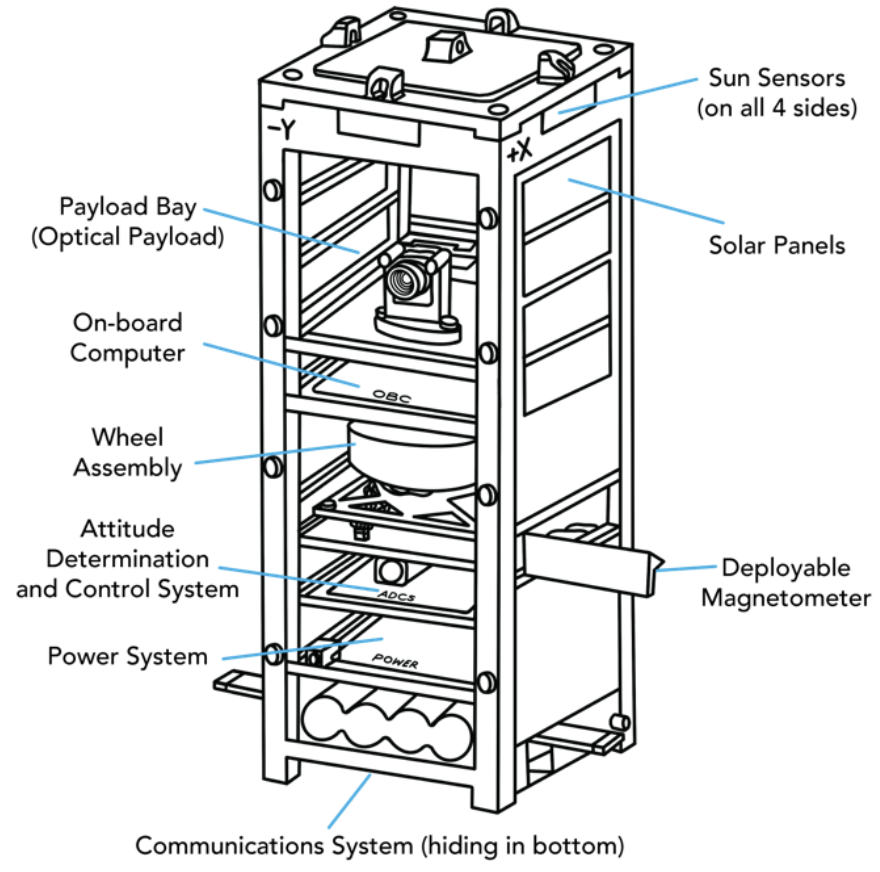
\includegraphics[width=0.75\linewidth]{images/SatDiagram.png}
    \caption{KISPE Satellite Learning Laboratory (SATLL) Diagram}
    \label{fig:diagram}
\end{figure}


\section{CAN Feature Extraction Algorithm}
\label{app:feature_extraction}

Algorithm~\ref{alg:features} gives the pseudocode for the sliding-window CAN feature extractor (implemented in \texttt{can\_feature\_engineering.py}). The extractor maintains per-ID rolling history and a global window deque of the most recent $W=50$ frames. All per-frame quantities are computed in $O(1)$ time; window statistics require one pass over the deque on each new frame, bounded by $O(W)$.

\begin{algorithm}[H]
\caption{CAN Sliding-Window Feature Extraction}
\label{alg:features}
\begin{algorithmic}[1]
\Require CAN frame stream $\mathcal{F}$; baseline $\mathcal{B}$: ID $\to$ expected DLC; window size $W$
\Ensure Per-frame feature vector $\mathbf{x} \in \mathbb{R}^{14}$ and label $y$
\State $\textit{window} \leftarrow$ empty deque (capacity $W$)
\State $\textit{prev}[\cdot] \leftarrow \emptyset$ \Comment{last frame per CAN ID}
\State $\textit{arrival}[\cdot] \leftarrow []$ \Comment{timestamp history per CAN ID}
\For{each frame $f = (\tau, \textit{id}, \textit{dlc}, \mathbf{d}, y)$}
    \State Append $f$ to $\textit{window}$; evict oldest if $|\textit{window}| > W$
    \State $\mathbf{p} \leftarrow \textit{prev}[\textit{id}]$ (or zeros if unseen)
    \State \textbf{// Payload structure}
    \State $x_1 \leftarrow \textit{id} / 2047$ \Comment{\texttt{can\_id\_norm}}
    \State $x_2 \leftarrow \textit{dlc}$
    \State $x_3 \leftarrow \mathrm{mean}(\mathbf{d})$;\; $x_4 \leftarrow \mathrm{std}(\mathbf{d})$
    \State $x_5 \leftarrow H(\mathbf{d})$ \Comment{Shannon entropy, bits}
    \State $x_6 \leftarrow \max(\mathbf{d}) - \min(\mathbf{d})$
    \State $x_7 \leftarrow \mathrm{popcount}(\mathbf{d} \oplus \mathbf{p}.\mathbf{d})$ \Comment{Hamming distance}
    \State $x_8 \leftarrow \sum_i |\mathbf{d}_i - \mathbf{p}.\mathbf{d}_i|$ \Comment{L1 payload delta}
    \State $x_9 \leftarrow \mathbf{1}[\textit{dlc} \neq \mathcal{B}[\textit{id}]]$ \Comment{\texttt{dlc\_anomaly}}
    \State $x_{10} \leftarrow \mathbf{1}[\textit{id} \in \mathcal{B}]$ \Comment{\texttt{id\_is\_known}}
    \State \textbf{// Temporal dynamics} (over \textit{window})
    \State $\Delta \leftarrow$ inter-arrival times of \textit{id} within \textit{window}
    \State $x_{11} \leftarrow \mathrm{mean}(\Delta)$
    \State $x_{12} \leftarrow |\{f' \in \textit{window} : f'.\textit{id} = \textit{id}\}| \;/\; (\textit{window\_span})$
    \State \textbf{// Bus topology} (over \textit{window})
    \State $x_{13} \leftarrow |\textit{window}| \;/\; (\textit{window\_span})$ \Comment{\texttt{bus\_load}}
    \State $x_{14} \leftarrow |\{\,f'.\textit{id} : f' \in \textit{window}\}|$ \Comment{\texttt{unique\_ids}}
    \State \textbf{yield} $(\mathbf{x}, y)$
    \State $\textit{prev}[\textit{id}] \leftarrow f$
\EndFor
\end{algorithmic}
\end{algorithm}


\begin{table}[t]
\caption{CAN IDS feature set (14 total). ``Window'' features are computed over the offline 50-frame sliding history; ``per-frame'' features are computed from the current frame and its same-ID predecessor.}
\label{tab:features}
\small
\begin{tabular}{@{}lp{5.2cm}@{}}
\toprule
\textbf{Feature} & \textbf{Description} \\
\midrule
\multicolumn{2}{@{}l}{\textit{Payload structure (per-frame)}} \\
\texttt{data\_mean}    & Mean of 8 payload bytes \\
\texttt{data\_std}     & Std.\ dev.\ of payload bytes \\
\texttt{data\_entropy} & Shannon entropy of payload \\
\texttt{data\_range}   & max$-$min of payload bytes \\
\texttt{dlc}           & Data length code (0--8) \\
\texttt{dlc\_anomaly}  & 1 if DLC deviates from trained baseline \\
\texttt{hamming\_dist} & Bit Hamming distance from previous same-ID frame \\
\texttt{payload\_delta}& L1 distance from previous same-ID payload \\
\midrule
\multicolumn{2}{@{}l}{\textit{Temporal dynamics (window)}} \\
\texttt{inter\_arrival\_mean} & Mean $\Delta t$ between same-ID frames \\
\texttt{id\_freq}             & This ID's message rate (msgs/s) \\
\texttt{bus\_load}            & Total bus message rate (msgs/s) \\
\midrule
\multicolumn{2}{@{}l}{\textit{Bus topology (window)}} \\
\texttt{can\_id\_norm} & Normalized 11-bit arbitration ID \\
\texttt{unique\_ids}   & Distinct IDs observed in window \\
\texttt{id\_is\_known} & 1 if this ID was seen during training \\
\bottomrule
\end{tabular}
\end{table}

% ============================================================
\section{Inference Algorithm}
\label{app:inference}

Algorithm~\ref{alg:inference} describes the onboard inference path executed by the STM32 firmware. The entire computation is stack-allocated; no heap calls occur. The feature buffer \texttt{feat[14]} (56~bytes) is populated by the CAN ISR or polling loop; \texttt{scale()} applies the precomputed z-score constants stored in flash; \texttt{tree\_predict()} traverses the 39-node decision tree using the exported C arrays.

\begin{algorithm}[t]
\caption{CAN IDS Inference (STM32)}
\label{alg:inference}
\begin{algorithmic}[1]
\Require CAN frame $f$; static flash arrays: \texttt{thresholds[N]}, \texttt{feature\_idx[N]},
         \texttt{children\_left[N]}, \texttt{children\_right[N]}, \texttt{leaf\_class[N]};
         static scaler arrays: \texttt{mean[14]}, \texttt{scale[14]}
\Ensure Alert flag $\hat{y} \in \{0,1\}$; clock cycles elapsed
\State \textbf{// Feature computation (CAN ISR context)}
\State \texttt{feat[14]} $\leftarrow$ \Call{compute\_features}{$f$, \textit{window}, \textit{baseline}}
\State \textbf{// Z-score normalization}
\For{$i \leftarrow 0$ \textbf{to} $13$}
    \State \texttt{feat[i]} $\leftarrow$ (\texttt{feat[i]} $-$ \texttt{mean[i]}) $/$ \texttt{scale[i]}
\EndFor
\State \textbf{// Tree traversal}
\State $\textit{node} \leftarrow 0$
\While{\texttt{children\_left[node]} $\neq -1$}  \Comment{not a leaf}
    \If{\texttt{feat[feature\_idx[node]]} $\leq$ \texttt{thresholds[node]}}
        \State $\textit{node} \leftarrow$ \texttt{children\_left[node]}
    \Else
        \State $\textit{node} \leftarrow$ \texttt{children\_right[node]}
    \EndIf
\EndWhile
\State $\hat{y} \leftarrow$ \texttt{leaf\_class[node]}
\If{$\hat{y} = 1$}
    \State \Call{ids\_raise\_alert}{$f$.\textit{id}, $\tau$} \Comment{publish via telemetry}
\EndIf
\State \Return $\hat{y}$
\end{algorithmic}
\end{algorithm}

% ============================================================
\section{Benchmark-to-CAN Encoding Algorithm}
\label{app:b2can}

Algorithm~\ref{alg:b2can} formalizes the tabular-to-CAN encoding used in the cross-domain experiment (Section~\ref{sec:methodology}). Each tabular sample of $F$ features is serialized as $1 + \lceil F/8 \rceil$ CAN frames: one meta frame carrying the sample index and binary label, followed by payload frames carrying min-max-scaled uint8 feature values packed 8 bytes at a time.

\begin{algorithm}[t]
\caption{Tabular-to-CAN Frame Encoding}
\label{alg:b2can}
\begin{algorithmic}[1]
\Require Tabular dataset $\{(\mathbf{x}_i, y_i)\}_{i=1}^{N}$; dataset code $c \in \{1,2\}$;
         inter-frame gap $\delta t = 1$~ms; meta CAN ID $\textit{id}_m$; base payload ID $\textit{id}_b$
\Ensure CAN frame stream with columns [\textit{timestamp}, \textit{can\_id}, \textit{dlc}, $d_0\ldots d_7$, \textit{label}]
\State $\mathbf{a} \leftarrow \min_i(\mathbf{x}_i)$;\; $\mathbf{b} \leftarrow \max_i(\mathbf{x}_i)$ \Comment{fit scaler on train split only}
\State $\tau \leftarrow 0$
\For{$i \leftarrow 1$ \textbf{to} $N$}
    \State $\mathbf{u} \leftarrow \mathrm{clip}\!\left(\left\lfloor 255 \cdot \tfrac{\mathbf{x}_i - \mathbf{a}}{\mathbf{b} - \mathbf{a}} \right\rceil,\, 0,\, 255\right)$ \Comment{uint8 encoding}
    \State \textbf{emit} meta frame: $(\tau,\; \textit{id}_m,\; 8,\;
           [i_{\&},\, i_{\gg 8},\, i_{\gg 16},\, y_i,\, \lceil F/8\rceil,\, c,\, \textit{split},\, 0])$
    \State $\tau \leftarrow \tau + \delta t$
    \For{$k \leftarrow 0$ \textbf{to} $\lceil F/8 \rceil - 1$}
        \State $\textit{chunk} \leftarrow \mathbf{u}[8k : \min(8k+8, F)]$ (zero-padded to 8 bytes)
        \State $\textit{dlc}   \leftarrow \min(8,\; F - 8k)$
        \State \textbf{emit} $(\tau,\; \textit{id}_b + k,\; \textit{dlc},\; \textit{chunk},\; y_i)$
        \State $\tau \leftarrow \tau + \delta t$
    \EndFor
\EndFor
\end{algorithmic}
\end{algorithm}

% ============================================================
\section{Feature Mathematical Definitions}
\label{app:feature_math}

Table~\ref{tab:feature_math} gives the precise mathematical definition of each of the 14 CAN features. $\mathcal{W}(t)$ denotes the set of frames in the sliding window at time $t$; $\mathcal{W}_{\textit{id}}(t)$ is the subset with matching arbitration ID. $\mathbf{d}(f)$ denotes the 8-byte payload vector of frame $f$; $\tau(f)$ its timestamp.

\begin{table}[t]
\caption{Mathematical definitions of the 14 CAN IDS features. $n = |\mathbf{d}|$; $H(\cdot)$ is Shannon entropy (bits); $W = |\mathcal{W}(t)|$.}
\label{tab:feature_math}
\small
\begin{tabular}{@{}ll@{}}
\toprule
\textbf{Feature} & \textbf{Definition} \\
\midrule
\texttt{can\_id\_norm}        & $\textit{id}\;/\;2047$ \\
\texttt{dlc}                  & $\textit{dlc}(f)$ \\
\texttt{data\_mean}           & $\frac{1}{n}\sum_i d_i$ \\
\texttt{data\_std}            & $\sqrt{\frac{1}{n}\sum_i(d_i - \bar{d})^2}$ \\
\texttt{data\_entropy}        & $H(\mathbf{d}) = -\sum_v p_v \log_2 p_v$ \\
\texttt{data\_range}          & $\max(\mathbf{d}) - \min(\mathbf{d})$ \\
\texttt{hamming\_dist}        & $\|\mathbf{d}(f) \oplus \mathbf{d}(f_{\textit{prev}})\|_{\mathrm{H}}$ \\
\texttt{payload\_delta}       & $\|\mathbf{d}(f) - \mathbf{d}(f_{\textit{prev}})\|_1$ \\
\texttt{dlc\_anomaly}         & $\mathbf{1}[\textit{dlc}(f) \neq \mathcal{B}[\textit{id}]]$ \\
\texttt{id\_is\_known}        & $\mathbf{1}[\textit{id} \in \mathcal{B}]$ \\
\texttt{inter\_arrival\_mean} & $\frac{1}{|\mathcal{W}_{\textit{id}}|-1}\sum \Delta\tau_{\textit{id}}$ \\
\texttt{id\_freq}             & $|\mathcal{W}_{\textit{id}}(t)|\;/\;\Delta\tau_{\mathcal{W}}$ \\
\texttt{bus\_load}            & $W\;/\;\Delta\tau_{\mathcal{W}}$ \\
\texttt{unique\_ids}          & $|\{\textit{id}(f') : f' \in \mathcal{W}(t)\}|$ \\
\bottomrule
\end{tabular}

\smallskip\footnotesize{$\Delta\tau_{\mathcal{W}} = \tau(f_{\text{newest}}) - \tau(f_{\text{oldest}})$ in window.}
\end{table}

% ============================================================
\section{Per-Attack-Type Detection Results}
\label{app:per_attack}

Table~\ref{tab:per_attack_full} gives per-attack-type recall for all pipeline variants that support per-class breakdown.

\begin{table}[t]
\caption{Per-attack-type recall (\%). Native CAN (Phase~4, $n_\text{test}=5{,}166$): four canonical satellite bus attack classes. NSL$\to$CAN (STM32 hardware, $n=48{,}000$ frames): all 30 attack types in the test split; FPR is a global figure for the configuration. Higher-recall attacks tend to alter payload statistics detectable via entropy/Hamming features.}
\label{tab:per_attack_full}
\small
\begin{tabular}{@{}lrr@{}}
\toprule
\textbf{Attack type} & \textbf{Recall (\%)} & \textbf{FPR (\%)} \\
\midrule
\multicolumn{3}{@{}l}{\textit{Native CAN IDS (Phase~4)}} \\
DoS          & 99.89 & 4.53 \\
Fuzzy        & 99.94 & 4.53 \\
Spoofing     & 100.0 & 4.53 \\
Replay       &  97.78 & 4.53 \\
\midrule
\multicolumn{3}{@{}l}{\textit{NSL$\to$CAN transfer on STM32 hardware}} \\
udpstorm     & 85.71 & 10.76 \\
xlock        & 57.14 & 10.76 \\
rootkit      & 54.76 & 10.76 \\
buffer\_overflow & 52.38 & 10.76 \\
mailbomb     & 45.21 & 10.76 \\
pod          & 41.90 & 10.76 \\
warezmaster  & 37.45 & 10.76 \\
snmpgetattack& 37.20 & 10.76 \\
guess\_passwd& 36.76 & 10.76 \\
ps           & 36.73 & 10.76 \\
processtable & 36.53 & 10.76 \\
smurf        & 36.01 & 10.76 \\
saint        & 35.64 & 10.76 \\
ipsweep      & 37.99 & 10.76 \\
back         & 35.04 & 10.76 \\
mscan        & 35.32 & 10.76 \\
neptune      & 35.24 & 10.76 \\
snmpguess    & 32.80 & 10.76 \\
portsweep    & 35.31 & 10.76 \\
httptunnel   & 31.11 & 10.76 \\
apache2      & 34.41 & 10.76 \\
satan        & 32.16 & 10.76 \\
phf          & 28.57 & 10.76 \\
land         & 28.57 & 10.76 \\
multihop     & 26.19 & 10.76 \\
named        & 25.00 & 10.76 \\
nmap         & 24.84 & 10.76 \\
teardrop     & 20.00 & 10.76 \\
sendmail     &  9.52 & 10.76 \\
xsnoop       &  9.52 & 10.76 \\
xterm        &  7.14 & 10.76 \\
\bottomrule
\end{tabular}
\end{table}

% ============================================================
\section{USB OTG Benchmark Wire Protocol}
\label{app:protocol}

Table~\ref{tab:protocol} documents the binary wire protocol used by \texttt{host\_inference\_runner.py} to drive the STM32 benchmark firmware. All multi-byte integers are little-endian.

\begin{table}[t]
\caption{USB OTG (CDC ACM) binary protocol between host runner and STM32 firmware. Sizes are in bytes.}
\label{tab:protocol}
\small
\begin{tabular}{@{}llrl@{}}
\toprule
\textbf{Direction} & \textbf{Message} & \textbf{Size} & \textbf{Contents} \\
\midrule
Host $\to$ MCU & Start      & 3  & \texttt{'S'} + uint16 $N$ (sample count) \\
Host $\to$ MCU & Features   & 56 & 14 $\times$ float32 feature vector \\
Host $\to$ MCU & Label      & 1  & uint8 ground-truth class (0/1) \\
MCU $\to$ Host & Sample result & 16 & uint8 pred, uint8 gt, uint32 cycles, \\
               &            &    & uint32 stack HWM, uint32 heap free, \\
               &            &    & int32 reserved \\
MCU $\to$ Host & Summary    & 64 & $N$, correct, TP, TN, FP, FN, \\
               &            &    & cyc\_min, cyc\_max, cyc\_sum\_hi, \\
               &            &    & cyc\_sum\_lo, stack\_hwm, energy\_nJ, \\
               &            &    & inf\_us\_mean, acc, prec, rec, f1, fpr \\
               &            &    & (18 fields: 11 $\times$ uint32 + 7 $\times$ float32) \\
\bottomrule
\end{tabular}
\end{table}

The MCU emits \texttt{[IDS]} prefixed log lines over the same USB CDC channel before the binary exchange; the host flushes these before initiating the sample stream. Cycle counts are measured with the ARM DWT cycle counter; stack high-water mark is measured using a canary fill pattern over a 1~KB task-stack region.

% ============================================================
\section{Quantization and Model Export}
\label{app:quantization}

Three numeric precision variants of the trained decision tree are exported as self-contained C headers: Float32 (32-bit IEEE thresholds), Int16 (linearly quantized 16-bit), and Int8 (8-bit). The quantized variants replace floating-point threshold comparisons with integer comparisons, eliminating FPU dependencies and enabling deployment on Cortex-M0 and M0+ cores.

All three formats are evaluated on the UNSW-NB15 test set (82K samples); results are shown in Table~\ref{tab:quant} and Figure~\ref{fig:quant_tradeoffs}. Float32 retains full detection quality (99.43\% recall, 85.24\% F1). Int16 maintains comparable recall (99.32\%) with slightly elevated FPR, at the cost of a 31\% increase in code size due to alignment overhead in the generated header. Int8 degrades markedly: recall falls to 66.4\% and F1 to 65.5\%, indicating that 8-bit precision is insufficient to represent the decision thresholds of a tree trained on z-scored floating-point features without a calibrated quantization pass. All three formats keep the model below 800~bytes, well within the flash budget of any STM32 variant.

\begin{table}[h]
\caption{Quantization comparison on UNSW-NB15 test set (82K samples).}
\label{tab:quant}
\small
\begin{tabular}{@{}lrrrrr@{}}
\toprule
\textbf{Format} & \textbf{Size} & \textbf{Acc.} & \textbf{Rec.} & \textbf{F1} & \textbf{Lat.} \\
                & (bytes)        & (\%)          & (\%)          & (\%)        & (\textmu s)   \\
\midrule
Float32 & 548 & 81.0 & 99.4 & 85.2 & 2.35 \\
Int16   & 731 & 77.0 & 99.3 & 82.6 & 6.32 \\
Int8    & 680 & 61.5 & 66.4 & 65.5 & 6.30 \\
\bottomrule
\end{tabular}
\end{table}

\begin{figure}[h]
  \centering
  \begin{subfigure}[b]{0.48\linewidth}
    \centering
    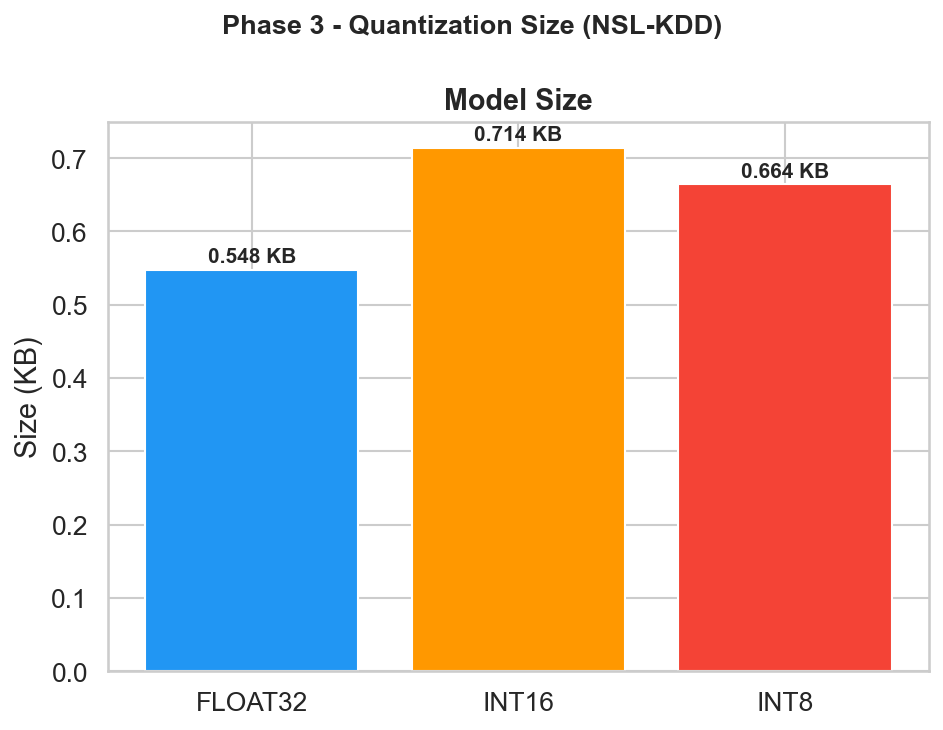
\includegraphics[width=\linewidth]{images/06b_quantization_size.png}
    \caption{Model size comparison.}
  \end{subfigure}
  \hfill
  \begin{subfigure}[b]{0.48\linewidth}
    \centering
    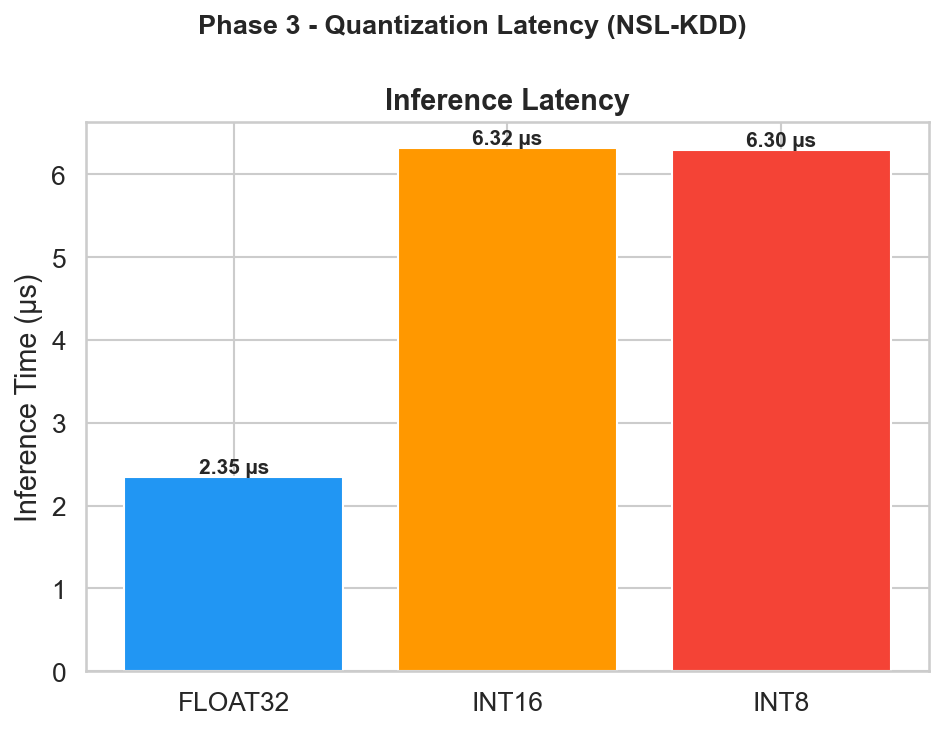
\includegraphics[width=\linewidth]{images/06c_quantization_latency.png}
    \caption{Inference latency comparison.}
  \end{subfigure}
  \caption{Quantization trade-offs for Float32, Int16, and Int8 variants.}
  \label{fig:quant_tradeoffs}
\end{figure}

% ============================================================
\section{Decision Tree Structure}
\begin{figure*}[h]
    \centering
    \includegraphics[width=\linewidth]{images/03_tree_structure_can.png}
    \caption{Trained TinyDecisionTree for the Satellite CAN IDS. Depth~5, 39~nodes, 20~leaves. Node color indicates class majority (blue = normal, orange = attack); numbers show Gini impurity, sample count, and class distribution. The tree is exported verbatim as static C arrays; inference traverses at most 5 comparisons per frame.}
    \label{fig:tree_structure}
\end{figure*}

\begin{figure}[t]
    \centering
    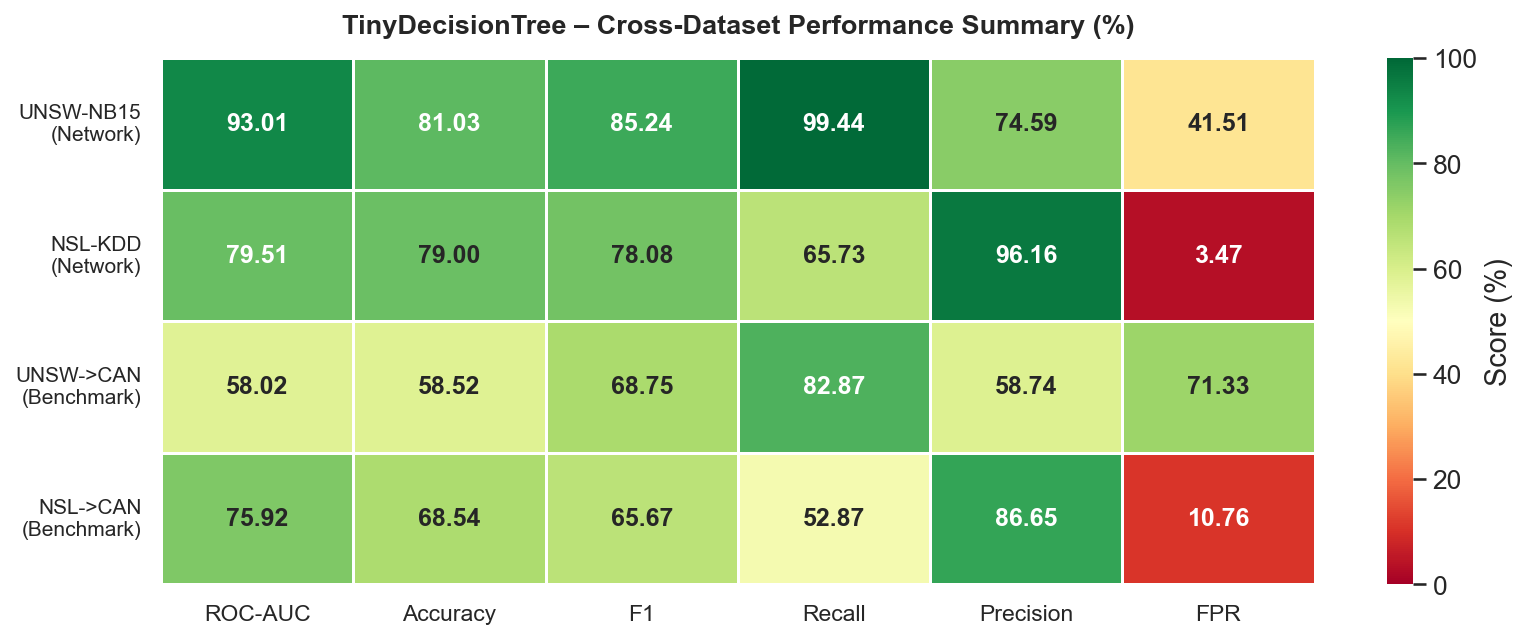
\includegraphics[width=\linewidth]{images/08_cross_dataset_heatmap.png}
    \caption{TinyDecisionTree performance heatmap across evaluation domains. Metrics are in percent; FPR is inverted (higher = lower FPR). The satellite CAN IDS achieves the strongest overall profile.}
    \label{fig:heatmap_summary}
\end{figure}

\end{document}
\endinput
%%
%% End of file `sample-manuscript.tex'.
